\appendix
\section{Appendix}

\subsection{More Visualization Results}

To provide a more comprehensive and intuitive understanding of Rex-Omni's capabilities, this section presents additional qualitative results across a wide range of visual perception tasks. These visualizations complement the quantitative results reported in the main paper, offering further insights into the model's performance in diverse and challenging scenarios. We showcase more visualization results for the following tasks:
\begin{itemize}
    \item Common and Long-tailed Object Detection (Figure \ref{fig:app_common_longtailed})
    \item Dense Object Detection (Figure \ref{fig:app_dense})
    \item  Object Referring (Figure \ref{fig:app_referring})
    \item  Object Pointing (Figure \ref{fig:app_pointing})
    \item Layout Grounding (Figure \ref{fig:app_layout})
    \item OCR (Optical Character Recognition) (Figure \ref{fig:app_ocr})
\end{itemize}

\begin{figure}[!h]     
    % \hspace*{-0.05\textwidth}
    \centering
    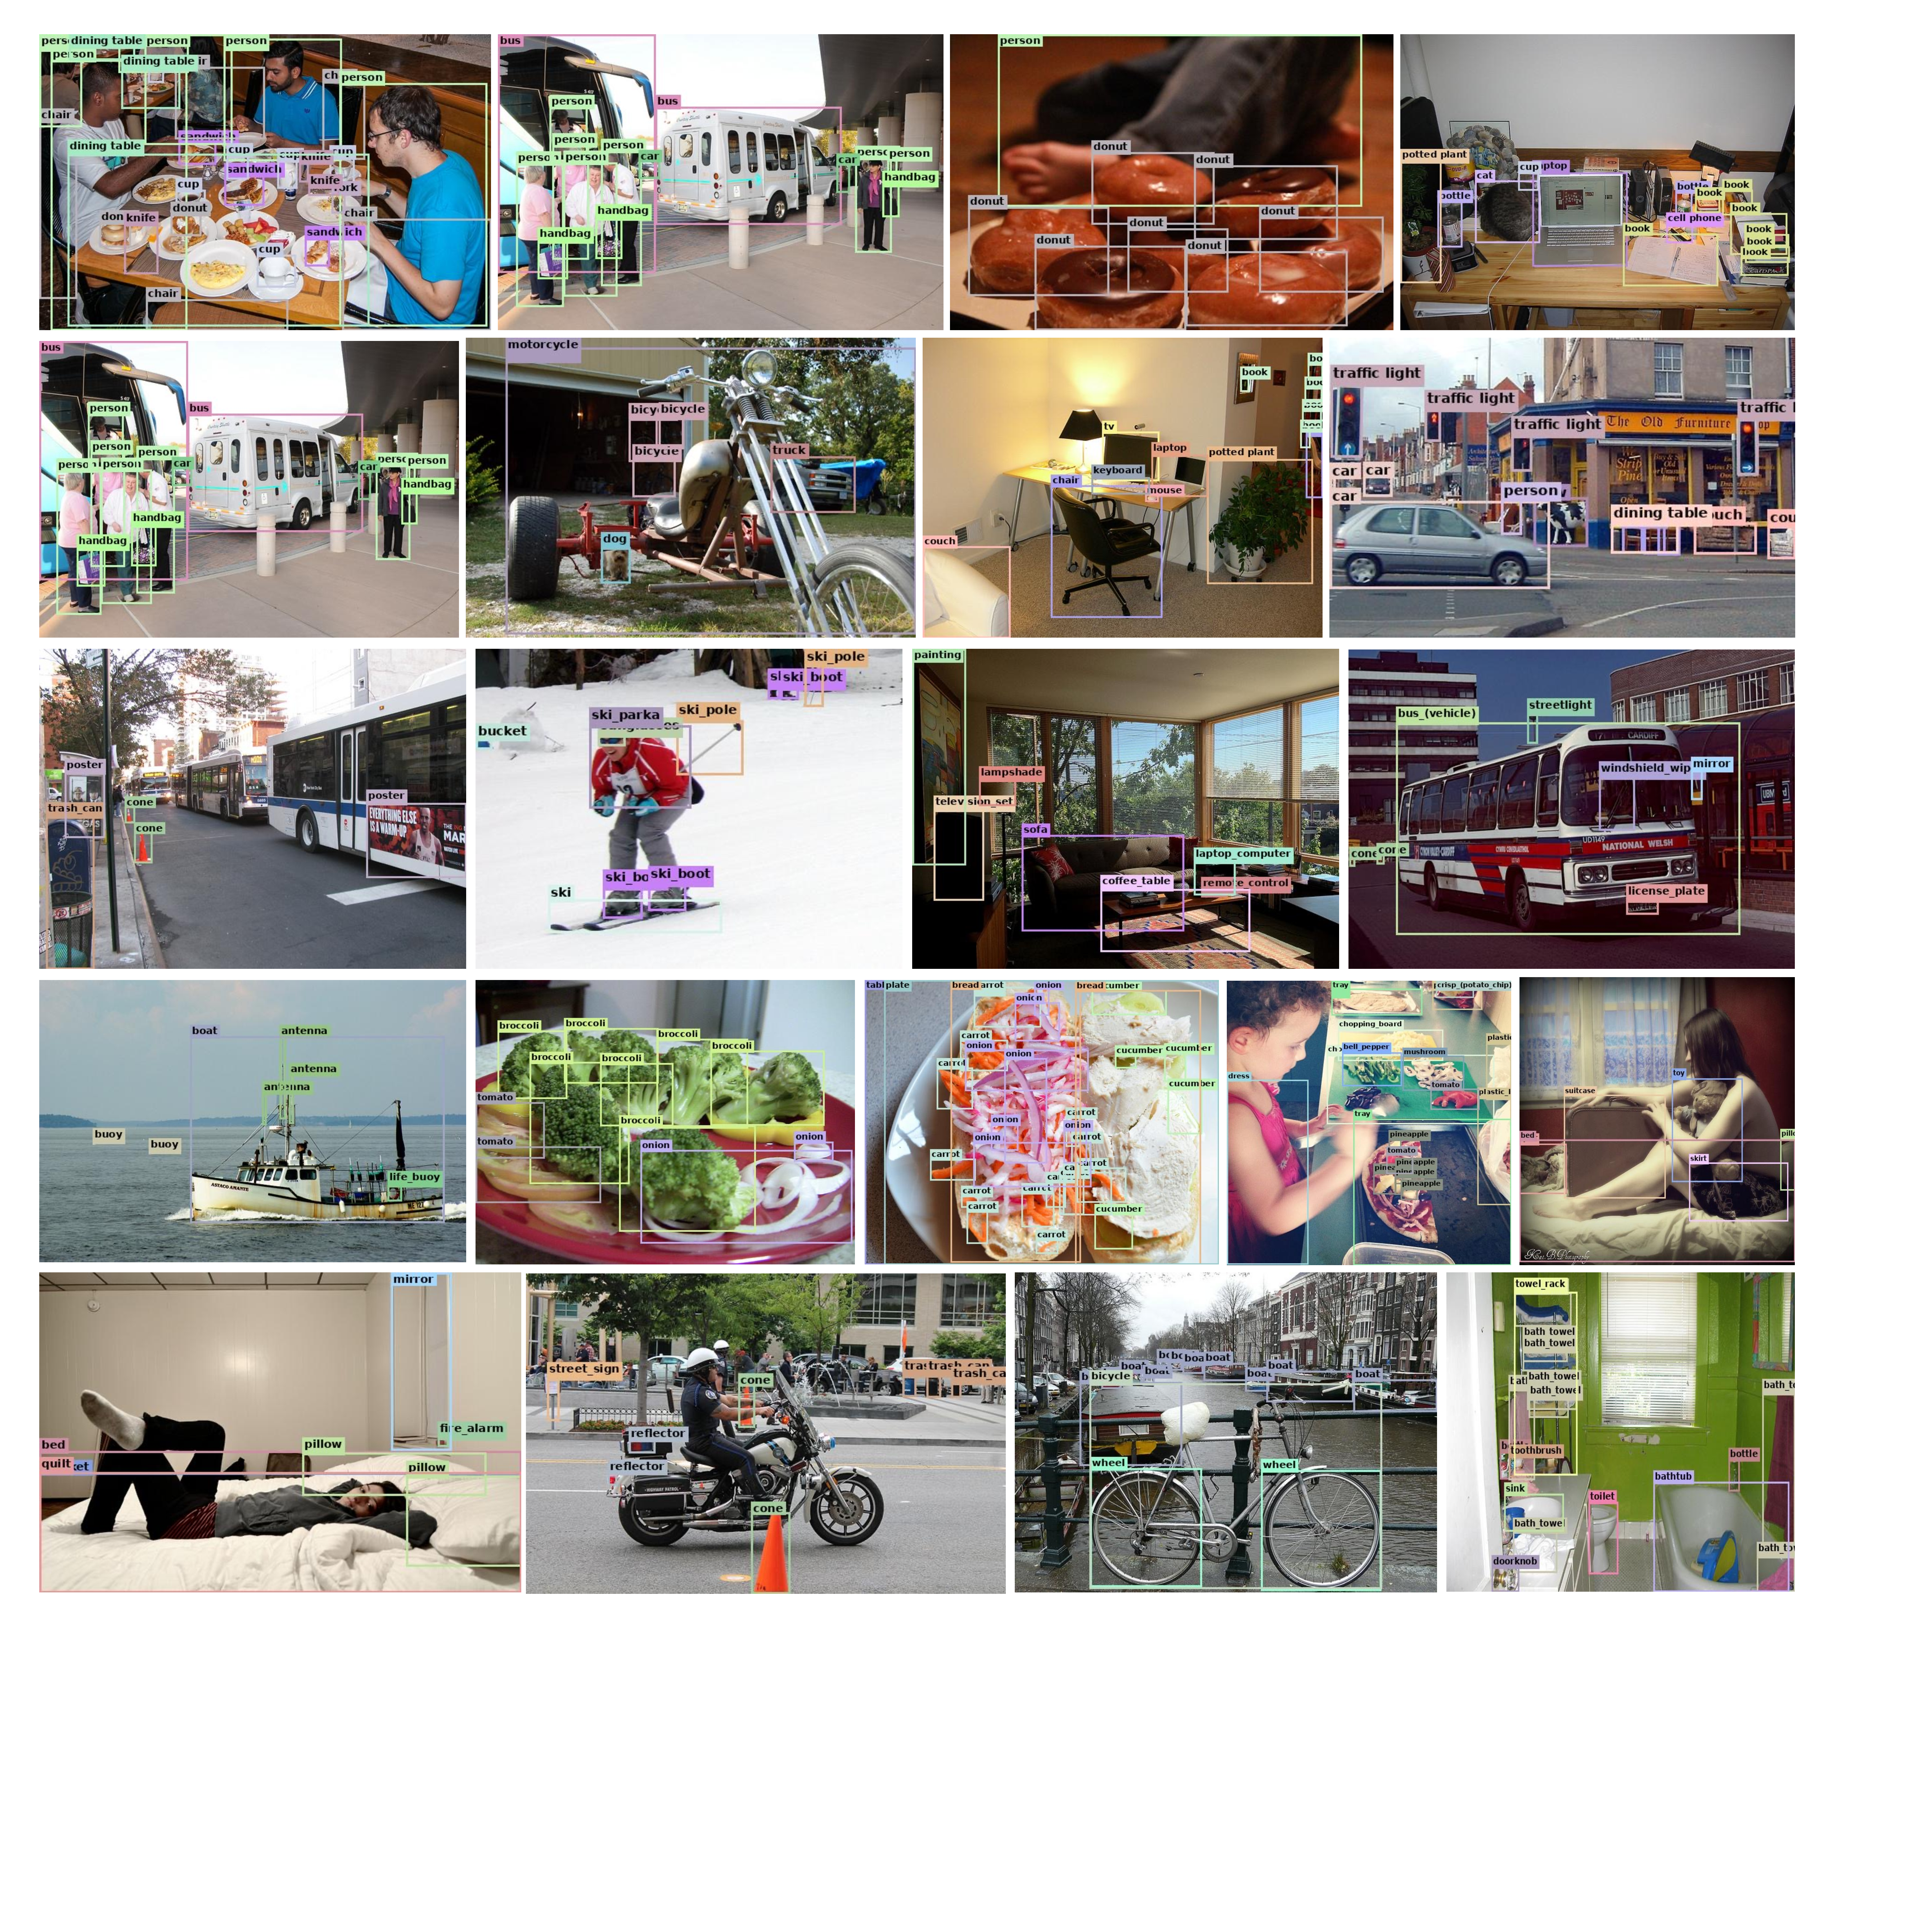
\includegraphics[width=0.8\textwidth]{appendix/common_longtailed.pdf}
    \captionsetup{justification=centering}
    \caption{Visualization results of Rex-Omni on common and long-tailed object detection task.}
    \label{fig:app_common_longtailed}
\end{figure}

\begin{figure}[t]     
    % \hspace*{-0.05\textwidth}
    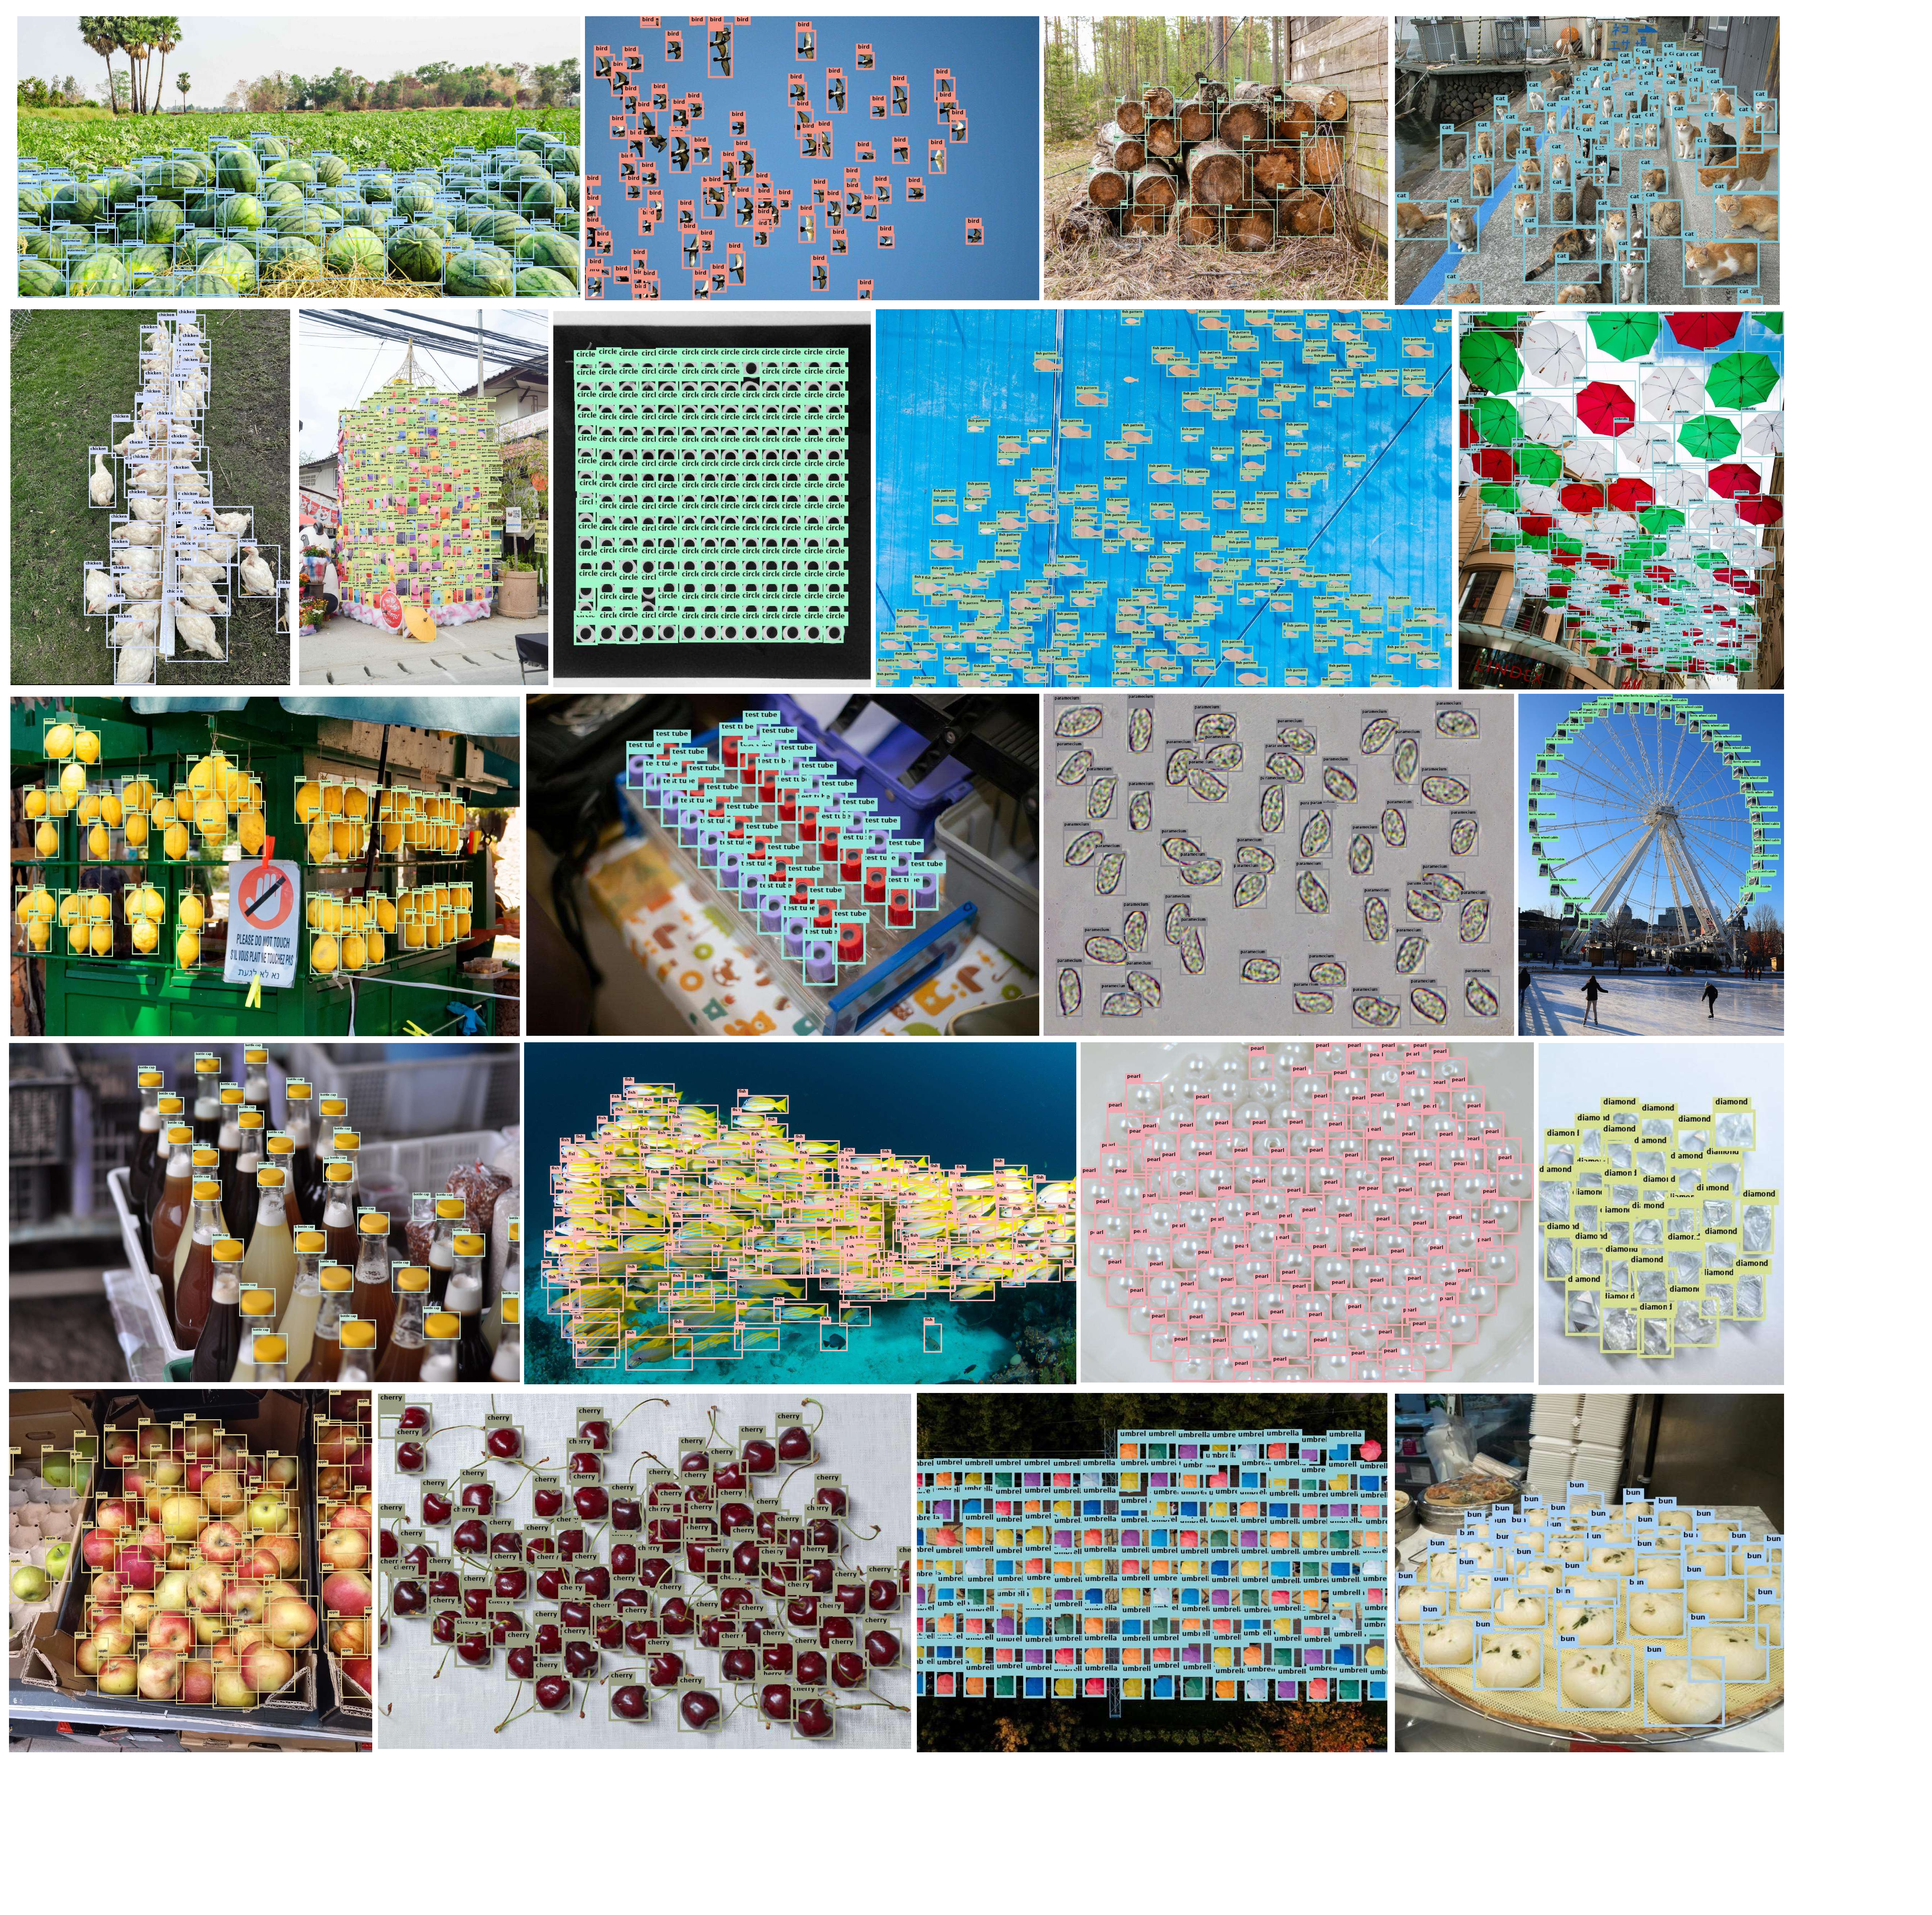
\includegraphics[width=1.0\textwidth]{appendix/dense.pdf}
    \captionsetup{justification=centering}
    \caption{Visualization results of Rex-Omni on dense object detection task.}
    \label{fig:app_dense}
\end{figure}

\begin{figure}[t]     
    % \hspace*{-0.05\textwidth}
    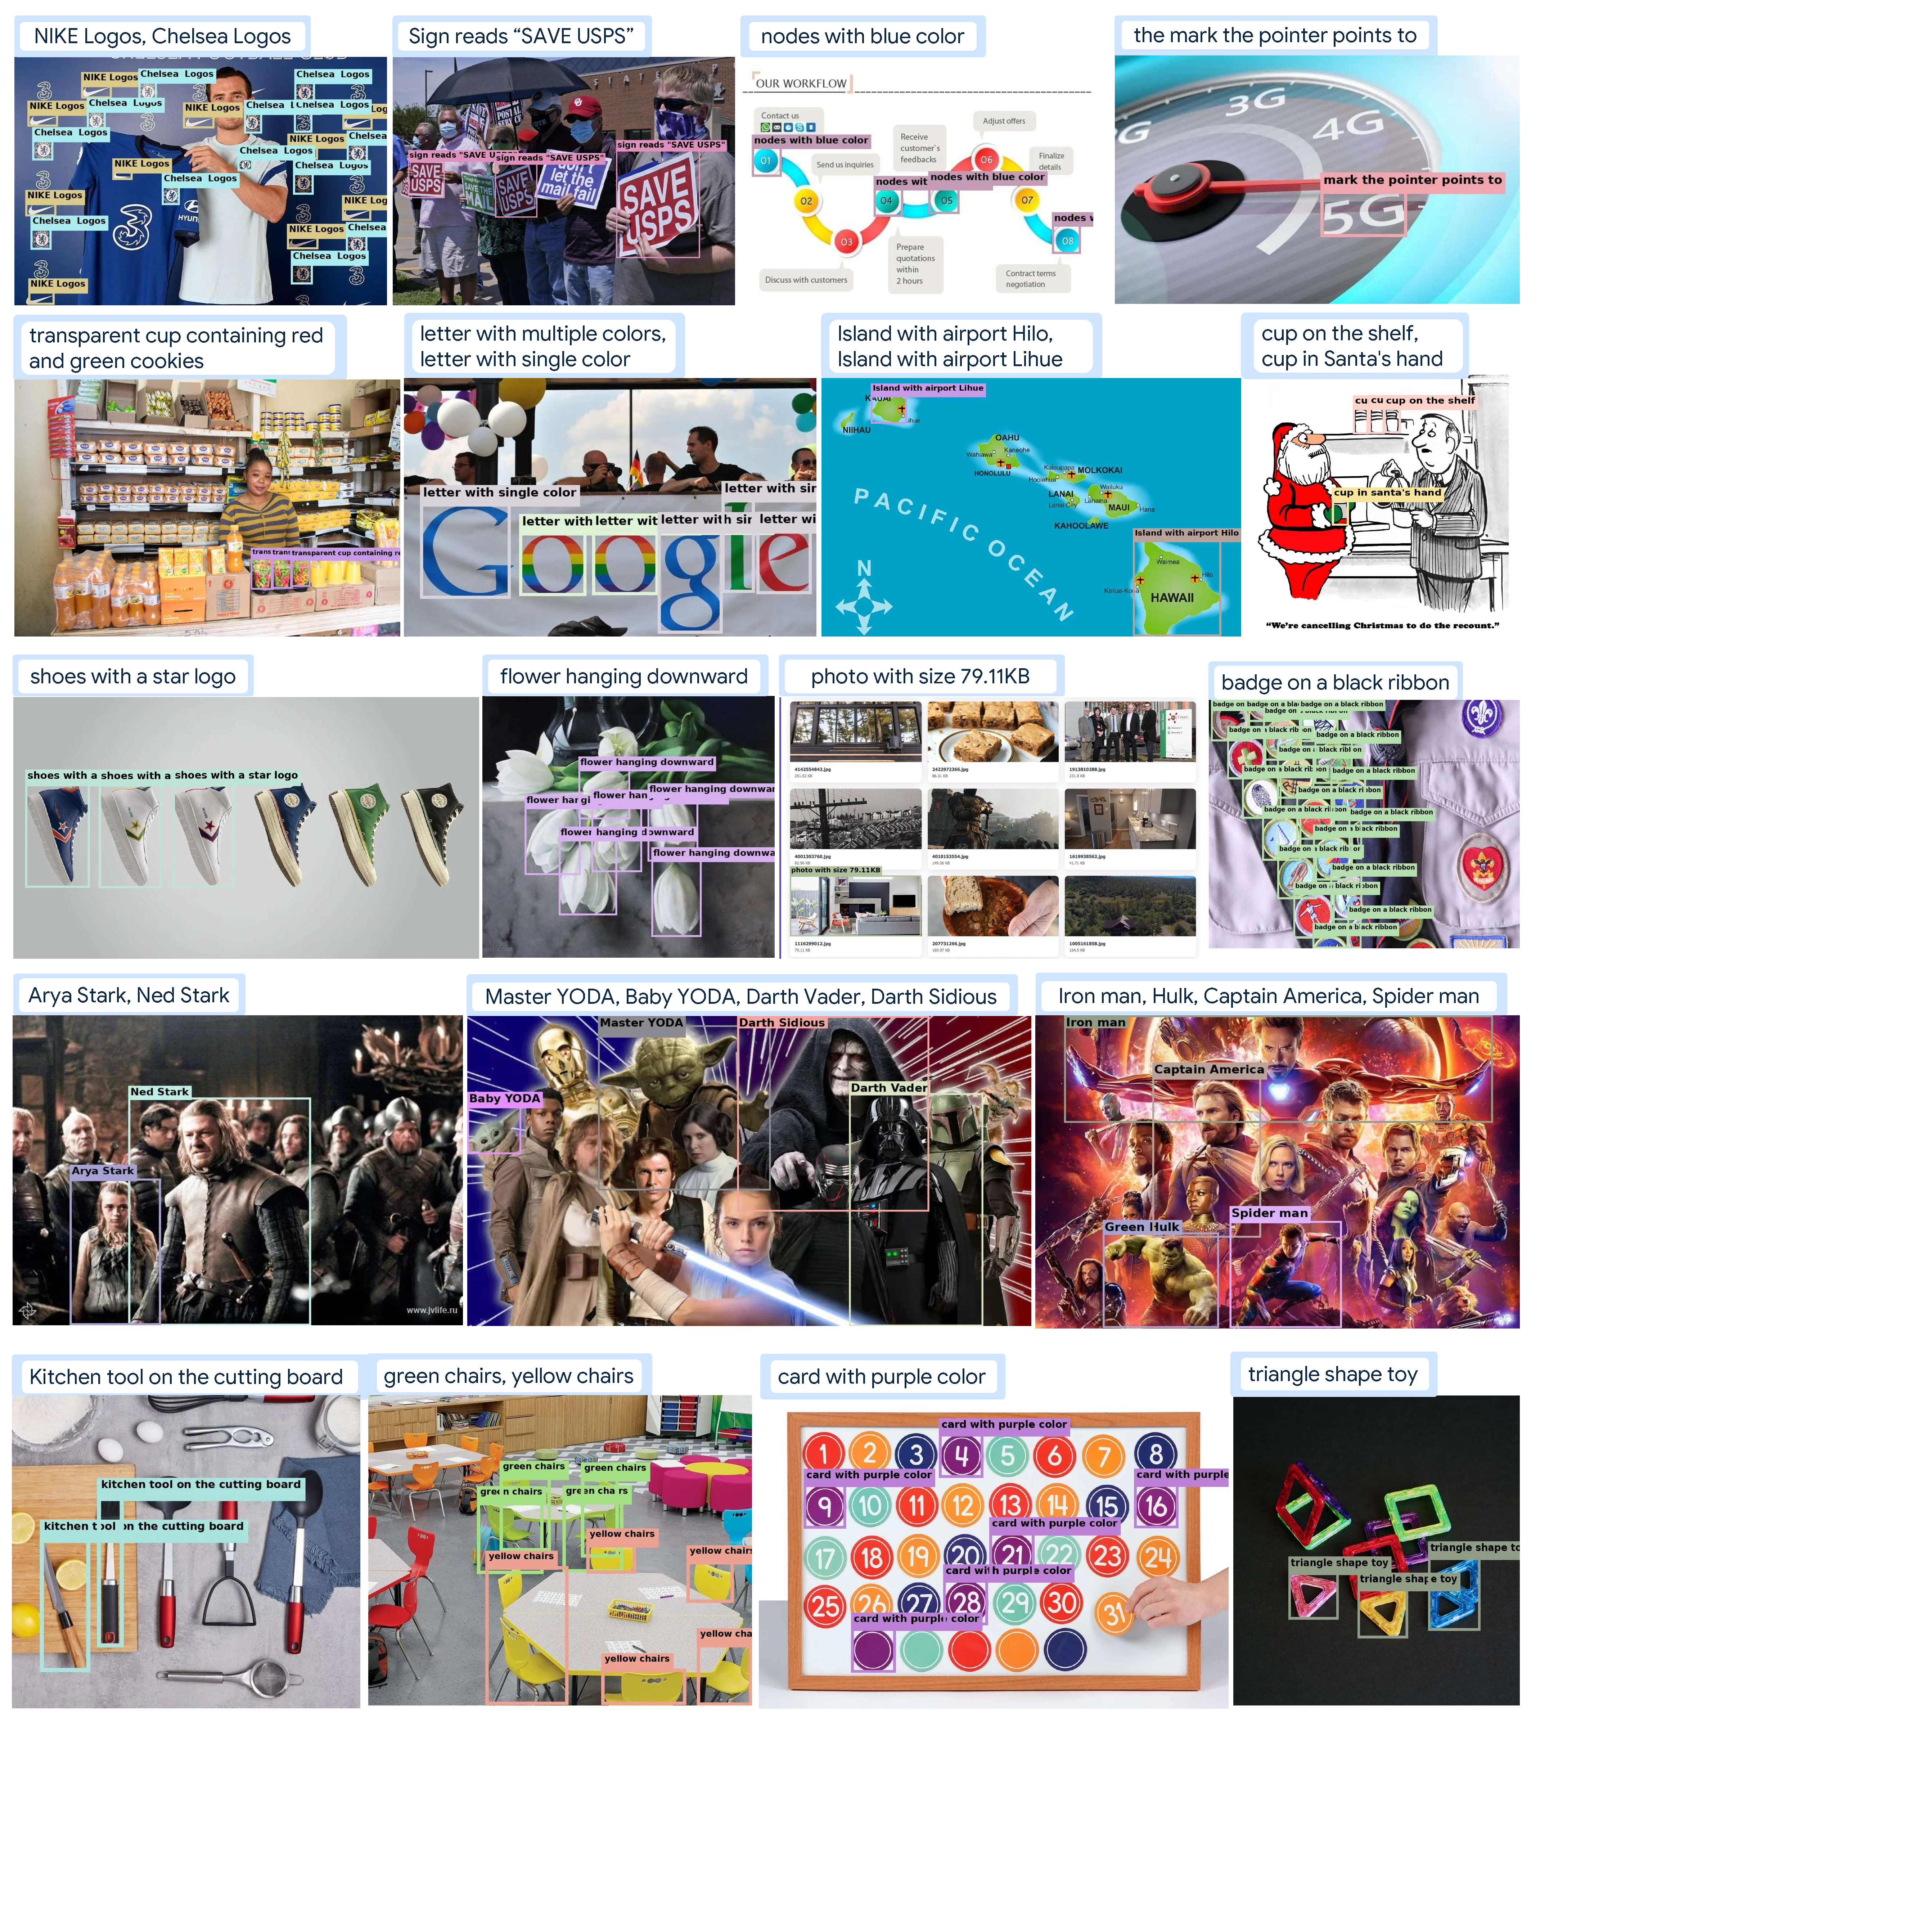
\includegraphics[width=1.0\textwidth]{appendix/referring.pdf}
    \captionsetup{justification=centering}
    \caption{Visualization results of Rex-Omni on object referring task.}
    \label{fig:app_referring}
\end{figure}

\begin{figure}[t]     
    % \hspace*{-0.05\textwidth}
    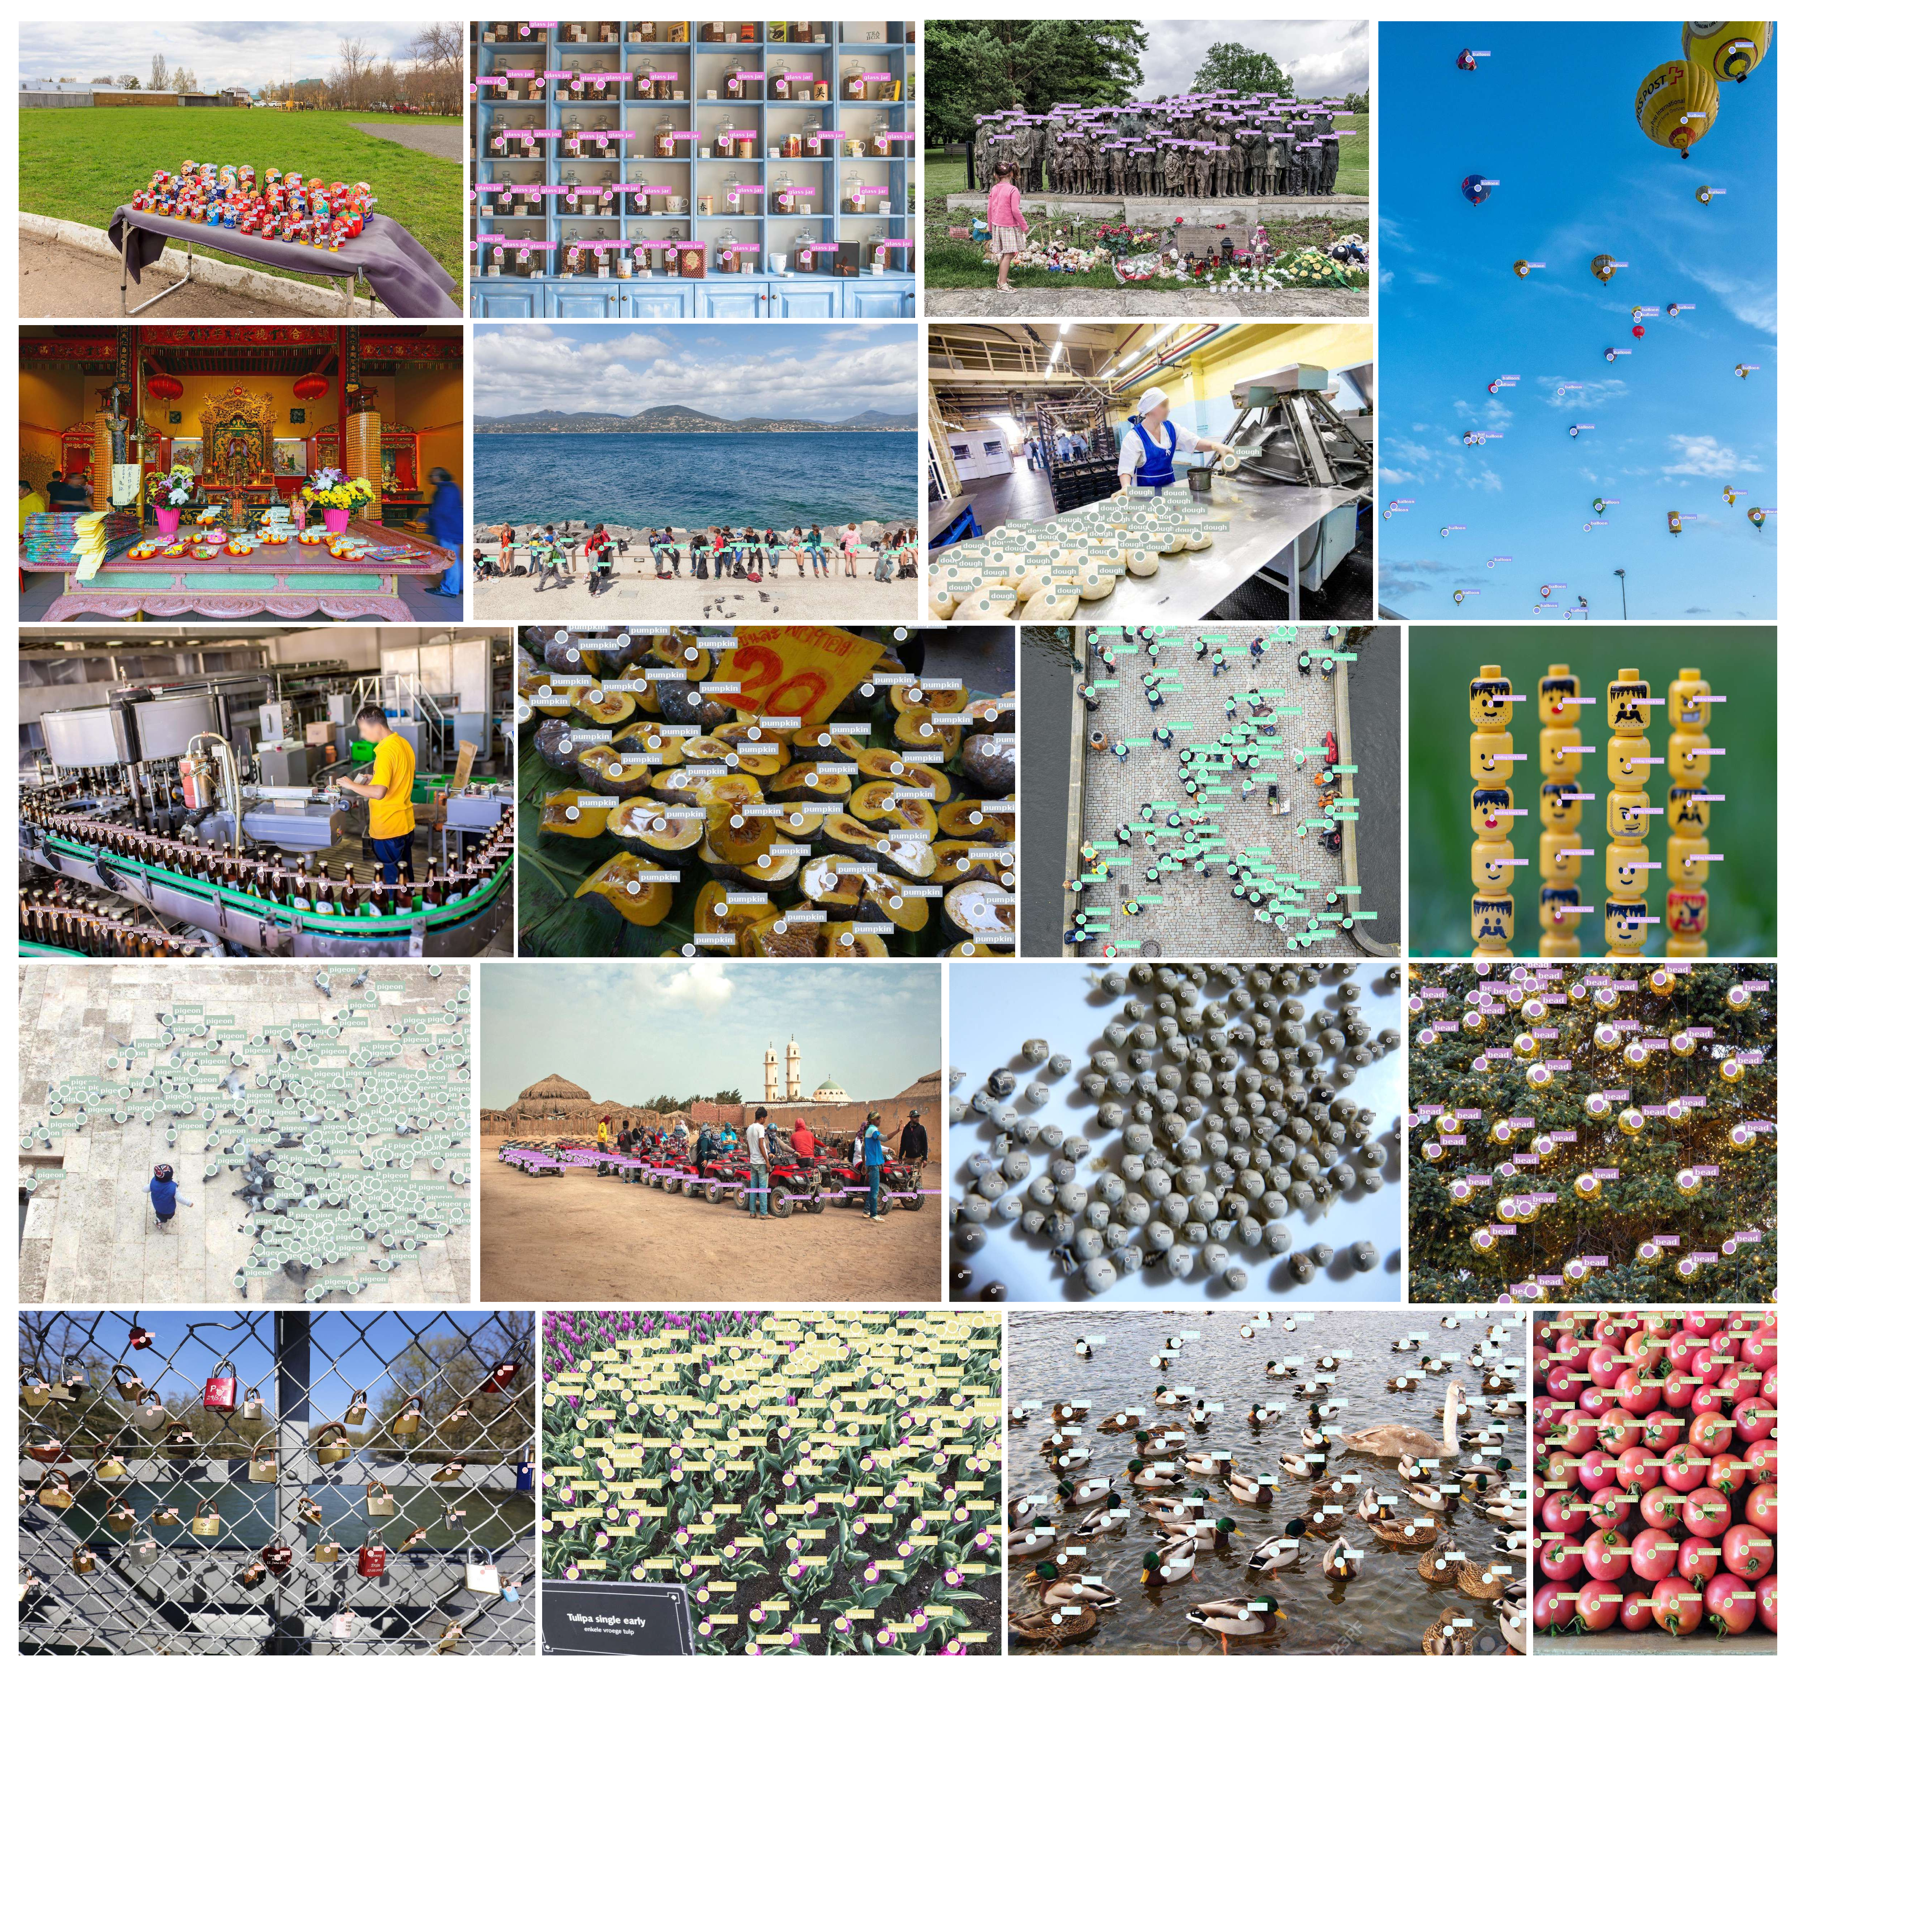
\includegraphics[width=1.0\textwidth]{appendix/pointing.pdf}
    \captionsetup{justification=centering}
    \caption{Visualization results of Rex-Omni on object pointing task.}
    \label{fig:app_pointing}
\end{figure}

\begin{figure}[t]     
    % \hspace*{-0.05\textwidth}
    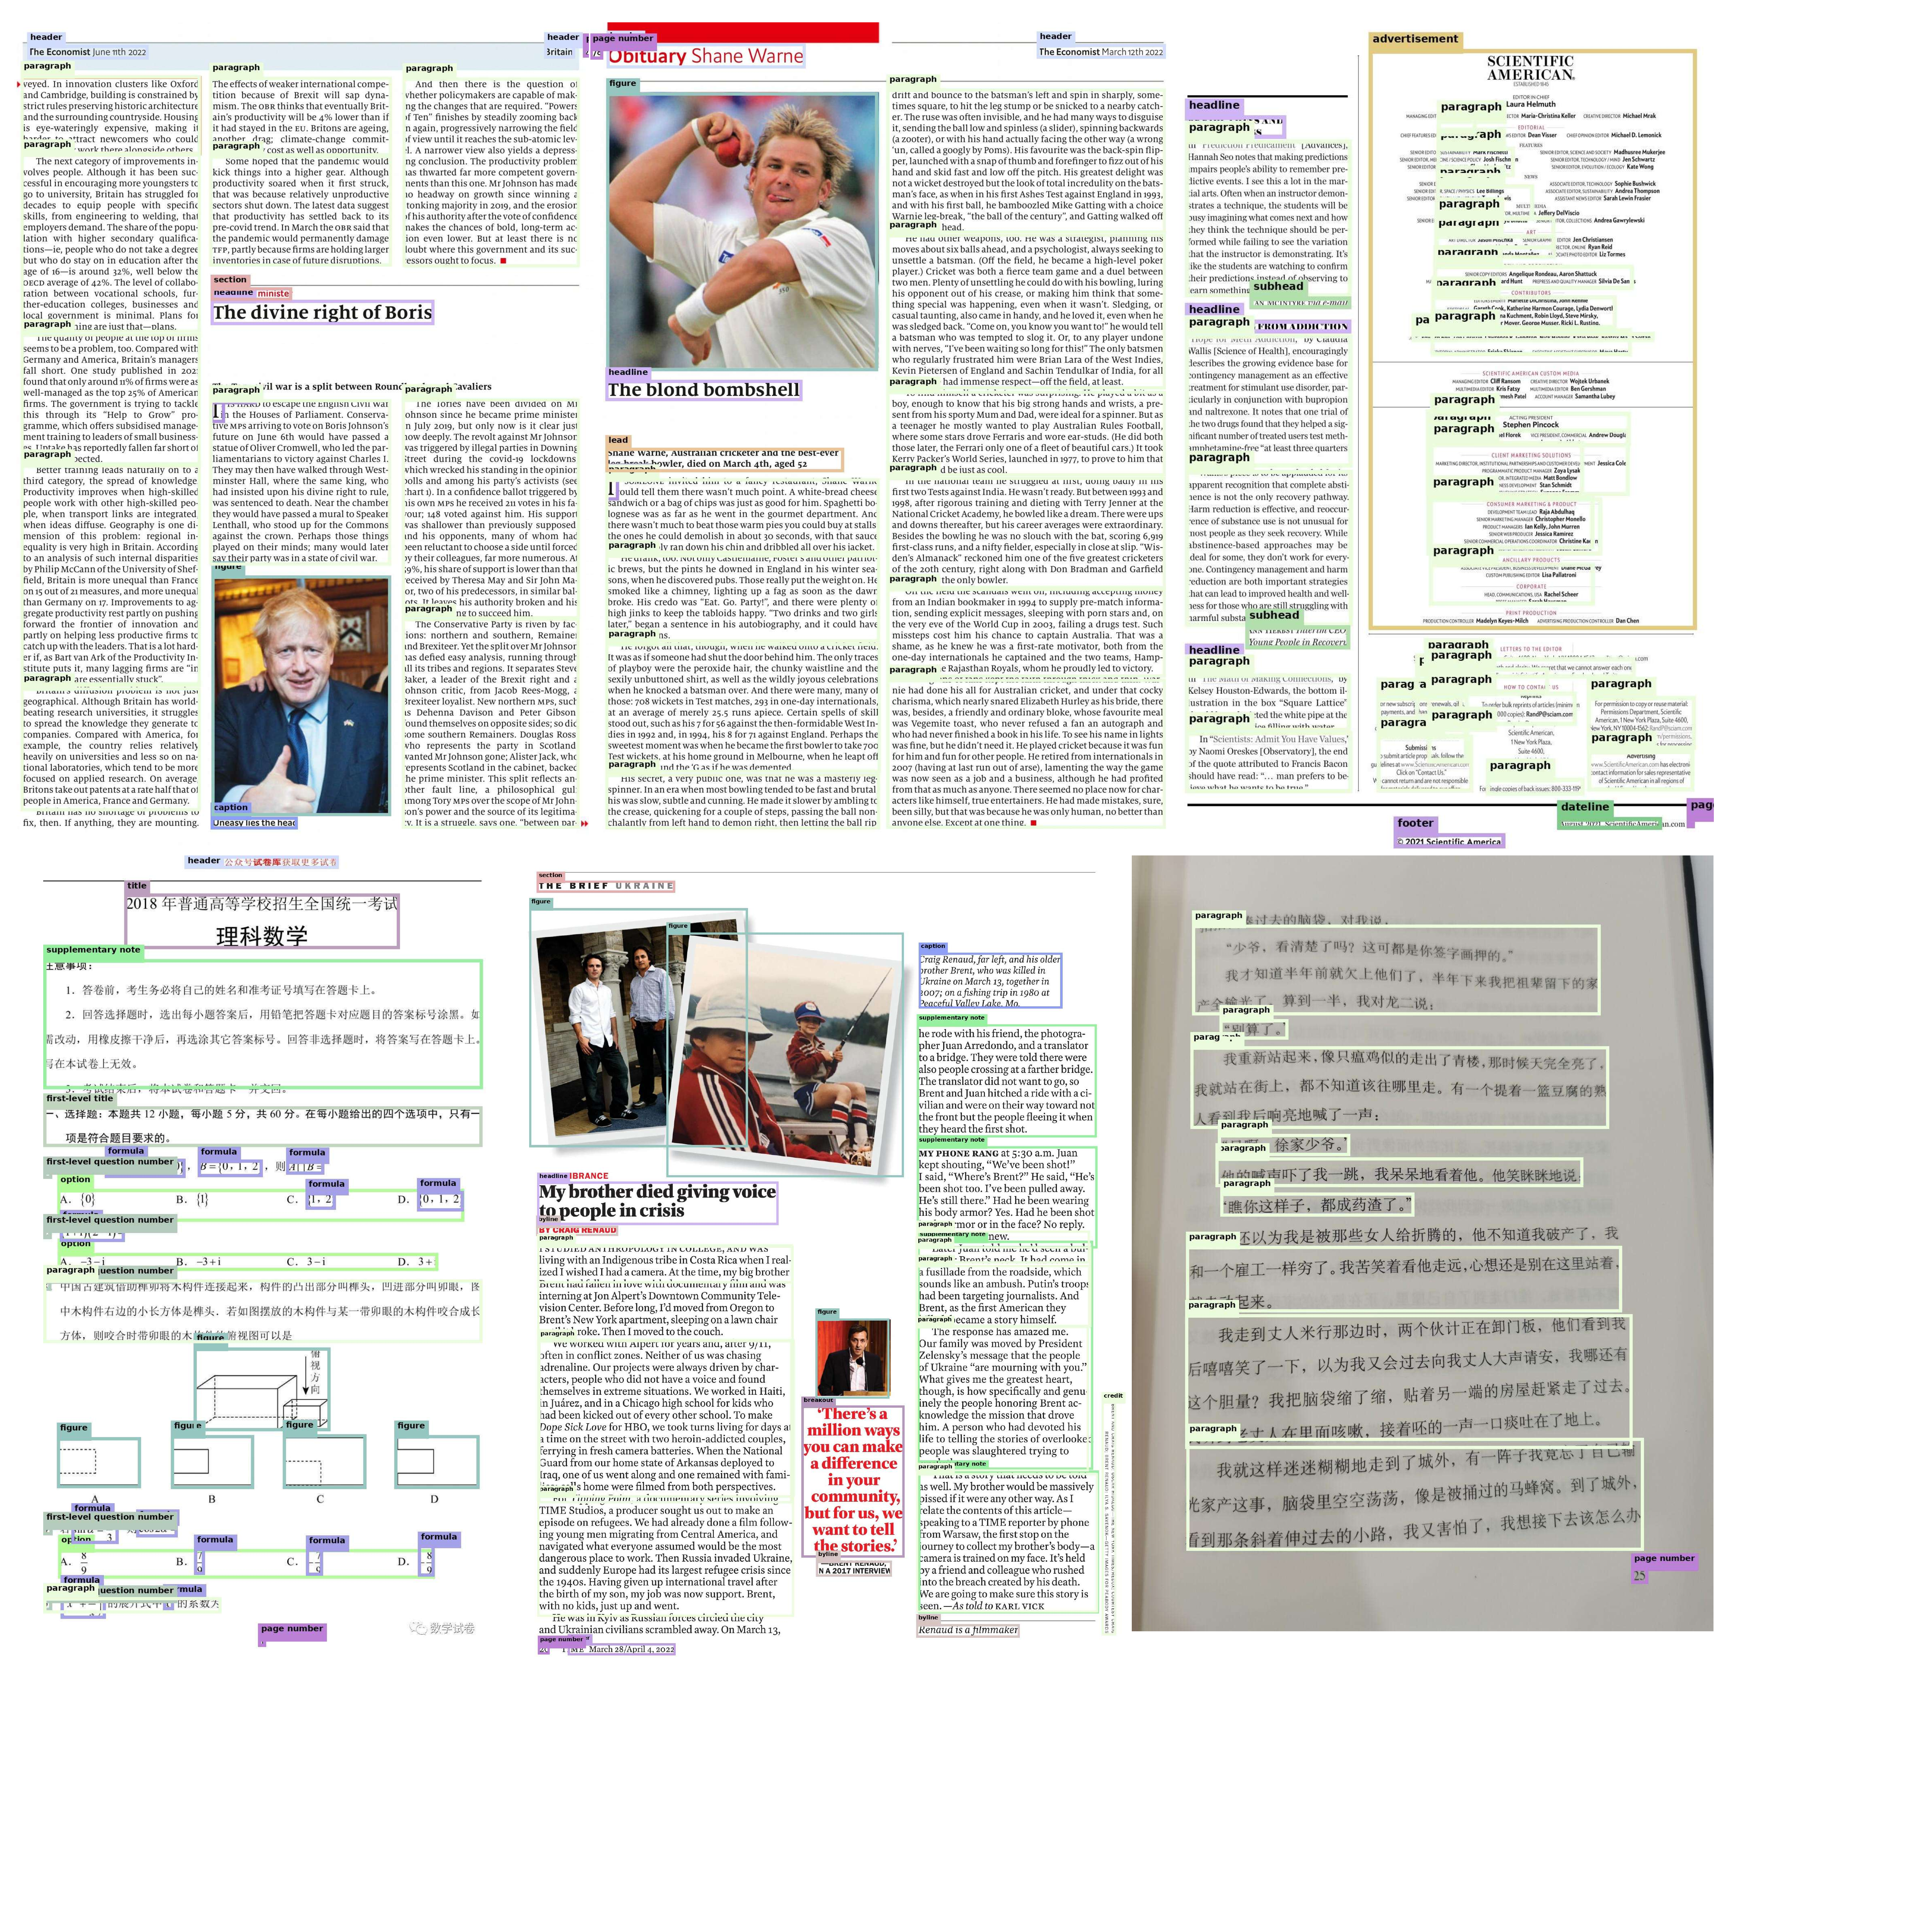
\includegraphics[width=1.0\textwidth]{appendix/layout.pdf}
    \captionsetup{justification=centering}
    \caption{Visualization results of Rex-Omni on layout grounding task.}
    \label{fig:app_layout}
\end{figure}

\begin{figure}[t]     
    % \hspace*{-0.05\textwidth}
    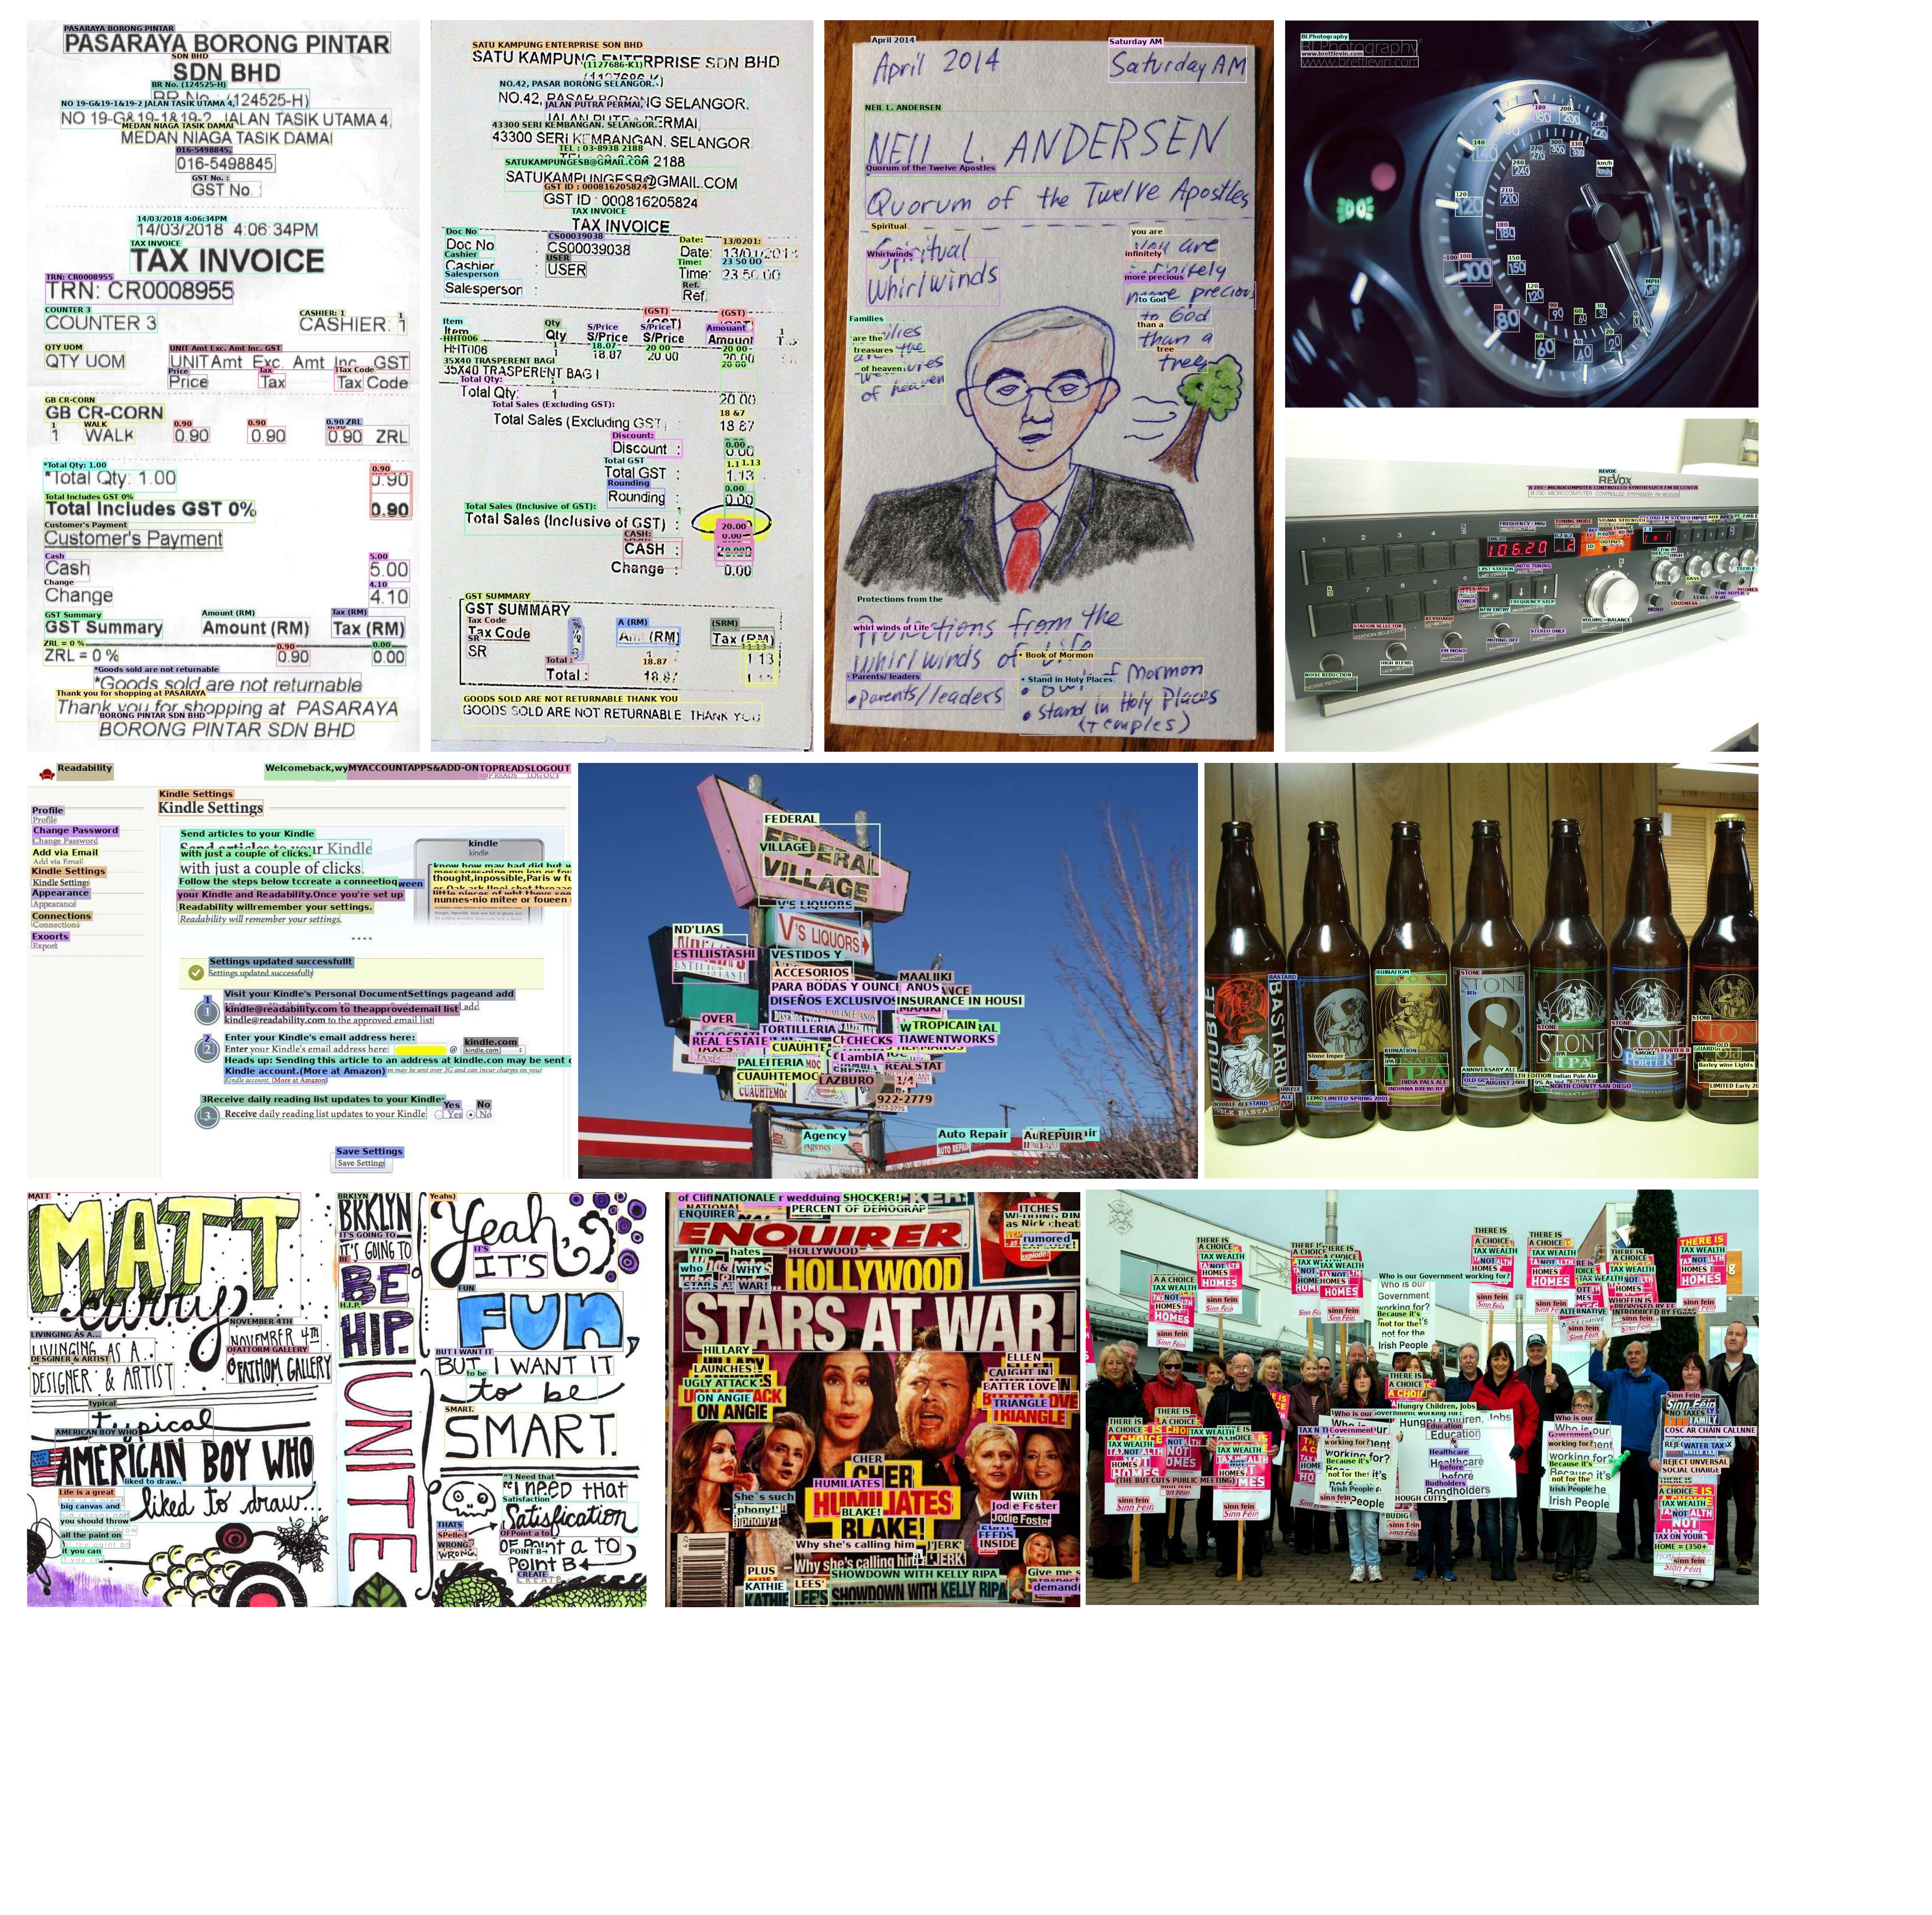
\includegraphics[width=1.0\textwidth]{appendix/ocr.pdf}
    \captionsetup{justification=centering}
    \caption{Visualization results of Rex-Omni on OCR task.}
    \label{fig:app_ocr}
\end{figure}






